% Adapted from Gelugor theme example by:
% LIM Lian Tze <liantze@gmail.com>, 2011
% http://liantze.penguinattack.org/latextypesetting

\documentclass{beamer}
\usetheme{UB}
\usepackage{wrapfig}
\usepackage{amsmath}
\usepackage{amsfonts}
\usepackage{graphicx}
\usepackage{algorithm2e}
\usepackage{verbatim}
\graphicspath{{./figures}{./figures/factorgraph}}

\DeclareMathOperator*{\argmin}{arg\,min}
\DeclareMathOperator*{\argmax}{arg\,max}
\newcommand{\vect}[1]{\mathbf{#1}}
\newcommand{\hvect}[1]{\bar{\vect{#1}}}
\newcommand{\uvect}[1]{\hat{\vect{#1}}}
\newcommand{\field}[1]{\mathbb{#1}}
\newcommand{\Real}[0]{\field{R}}
\newcommand{\map}{\vect{x}}
\newcommand{\meas}{z}
\newcommand{\measurements}{\vect{\meas}}
\newcommand{\pose}{g}
\newcommand{\poses}{\vect{\pose}}
\newcommand{\unaryminus}{\scalebox{0.5}[0.5]{\( - \)}}
\newcommand{\prevtime}{1:t\unaryminus1}
%\newcommand{\pastobs}{\sigma_{\prevtime}}
\newcommand{\pastobs}{\measurements_{1:t\unaryminus1}, \poses_{1:t\unaryminus1}}
\newcommand{\remaining}{\measurements_{\prevtime}, \poses_{\prevtime}}
\providecommand{\DontPrintSemicolon}{\dontprintsemicolon} % difference in versions

%% Use any fonts you like.
%\usepackage{helvet}

\title{Occupancy grid mapping with modern MAP inference algorithms}
%\subtitle{A subtitle}
\author{Vikas Dhiman}
\date{\today}
\institute{\url{vikasdhi@buffalo.edu}}

% Adjust your address/title page text with the \address command
\renewcommand{\address}
{
	Vision and Perceptual Machines Lab\\
}

%% Uncomment to change the pic on the title frame
%% Sizing and placement currently only look good with landscape orientation, not portrait
%\renewcommand{\titlepic}{some_other_title_frame_image}

\begin{document}

\begin{frame}
\titlepage
\end{frame}


\section{Introduction}

% \begin{frame}
% \frametitle{Occupancy Grid to factor graph}
% 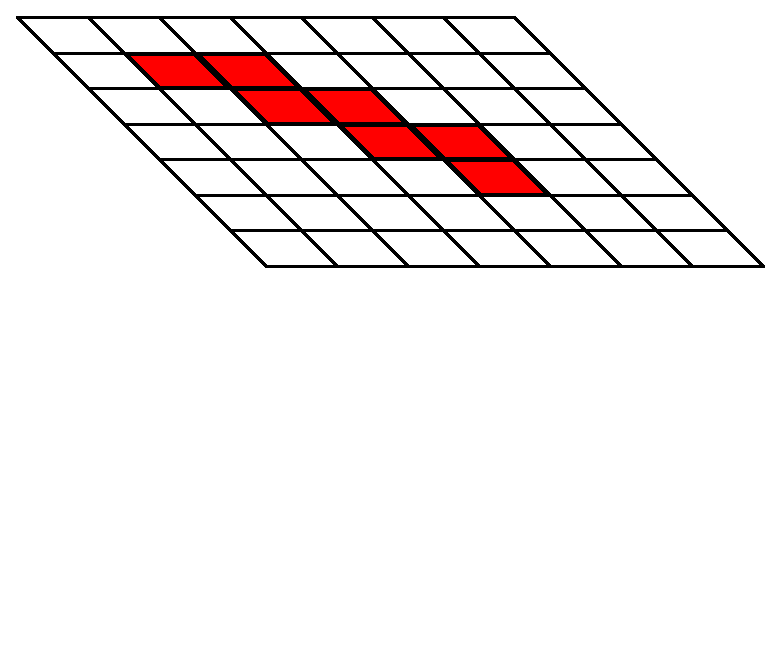
\includegraphics[width=\textwidth]{figures/factorgraph/fg0.pdf}
% \end{frame}

\begin{frame}
\frametitle{Occupancy Grid to factor graph}
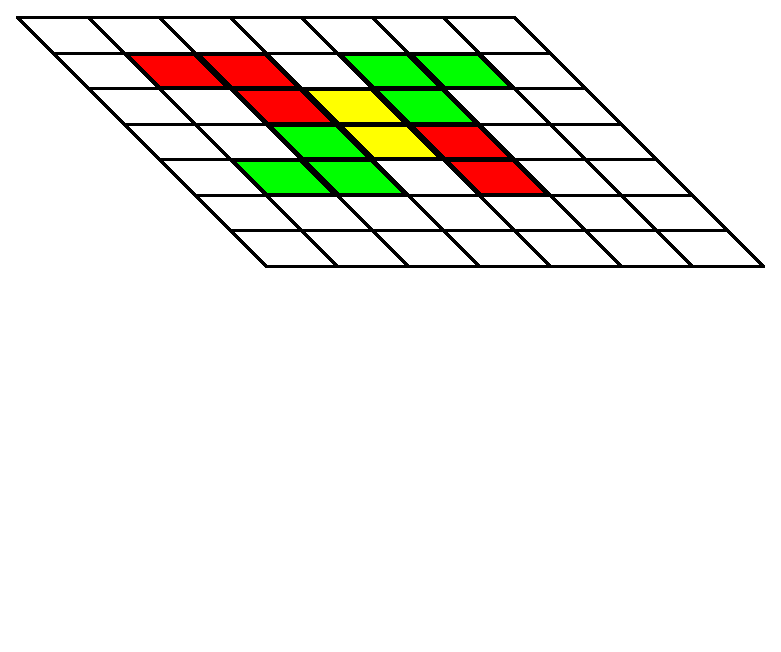
\includegraphics[width=\textwidth]{figures/factorgraph/fg1.pdf}
\end{frame}

\begin{frame}
\frametitle{Occupancy Grid to factor graph}
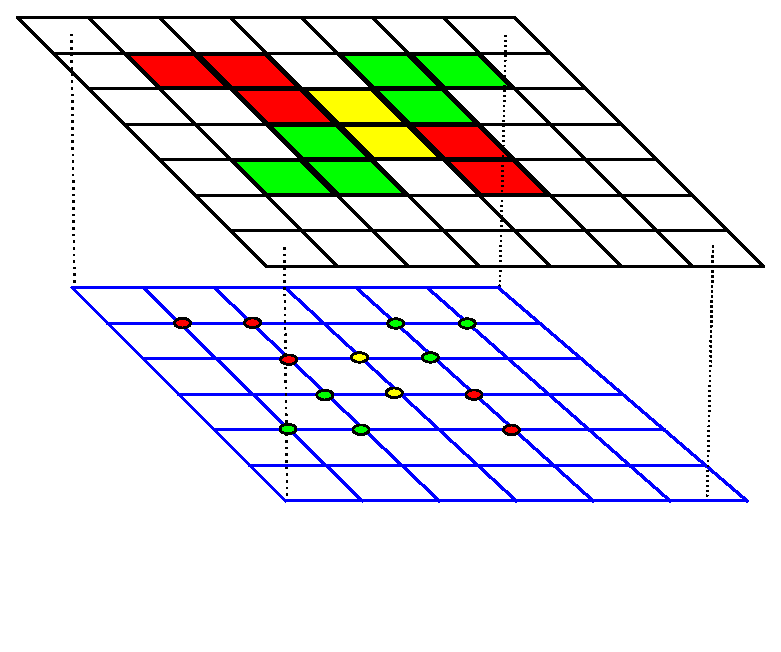
\includegraphics[width=\textwidth]{figures/factorgraph/fg2.pdf}
\end{frame}

\begin{frame}
\frametitle{Notation}

\begin{columns}
  \begin{column}{0.7\textwidth}
    \begin{itemize}
      \item $\map_i$ = Occupancy of $i^{th}$ cell of map $\map$
      \item $\pose_f$ = Pose (position + angle) of $f^{th}$ laser observation
      \item $\meas_f$ = Range observation given by $f^{th}$ laser observation
      %\item $f_t = f(m, x_t)$\\
        = First occupied cell in map $m$ that blocks laser for $t^{th}$ observation
    \end{itemize}
  \end{column}
  \begin{column}{0.3\textwidth}
    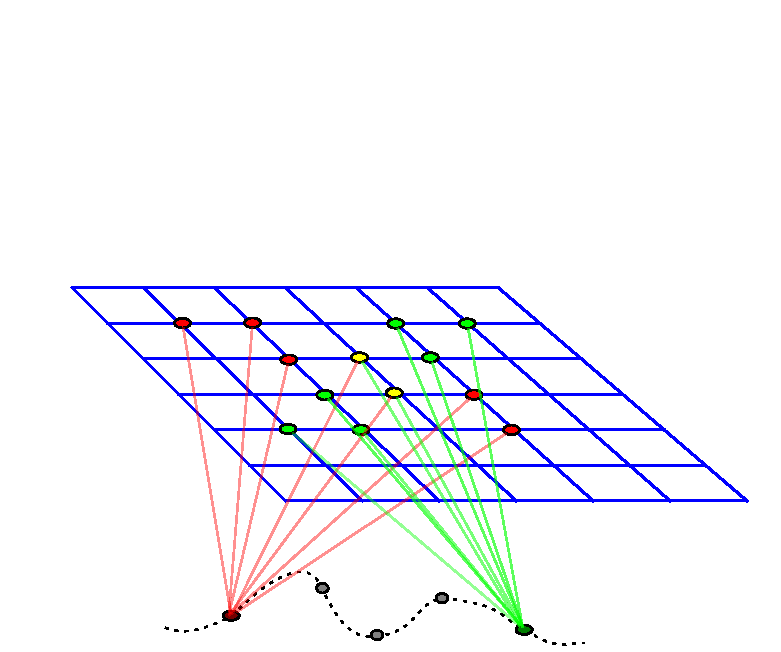
\includegraphics[trim=0in 0in 0in 2in, width=\textwidth]{figures/factorgraph/fg3.pdf}
  \end{column}
\end{columns}
\end{frame}

\begin{frame}
  \frametitle{Inverse sensor model:Assumption}
  % \begin{figure}
  %   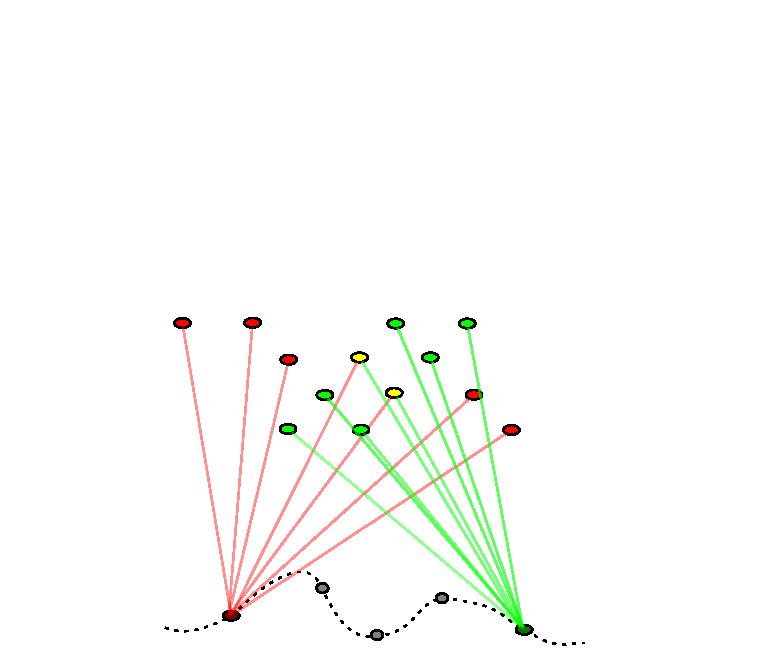
\includegraphics[trim=0in 0in 0in 2in, width=0.3\textwidth]{figures/factorgraph/fg_two_assumption.pdf}
  % \end{figure}
  \begin{align}
    p(\map|\measurements, \poses) &= \prod_{1 \le i \le N} p(x_i|\measurements, \poses)
  \end{align}
\end{frame}
\begin{frame}
  \frametitle{Inverse sensor model:Cell probability}
  \begin{align}
    p(x_i|\measurements, \poses) &= \frac{p(\meas_t, \pose_t|x_i, \remaining)p(x_i|\remaining)}
    {p(\meas_t, \pose_t|\remaining)}\\
  \end{align}
  Assuming static world $p(z_t, g_t|x_i, \remaining) = p(z_t, g_t|x_i)$
  \begin{align}
    p(x_i|\measurements, \poses) 
 % We can uncomment this detail if we need full derivation.
    &= p(\meas_t, \pose_t|x_i)\frac{p(x_i|\remaining)} {p(\meas_t, \pose_t|\remaining)}\\
    &= \frac{p(x_i|\meas_t, \pose_t)p(\meas_t,\pose_t)} {p(x_i)}\frac{p(x_i|\remaining)}{p(\meas_t, \pose_t|\remaining)}\\
    &= \frac{1}{Z'}\frac{p(x_i|\meas_t, \pose_t)}{p(x_i)}p(x_i|\remaining)\\
    &= \frac{1}{Z'p^{t-1}(x_i)}\prod_{1\le f \le t} p(x_i|\meas_f, \pose_f)
    \label{eq:assumeindependence}
  \end{align}
\end{frame}

\begin{frame}
  \frametitle{Forward sensor model}
  % \begin{figure}
  %   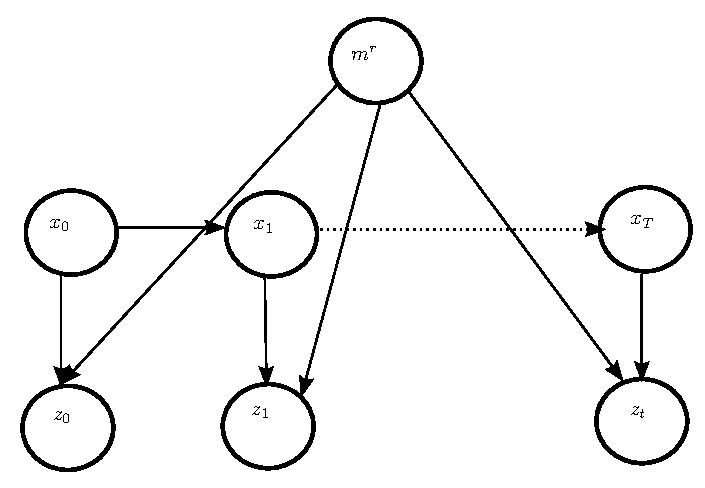
\includegraphics[width=0.3\textwidth]{figures/mrf_model_wrapper.pdf}
  % \end{figure}
  \begin{align}
    p(\map | \measurements, \poses) &= p(\map | \remaining, z_t, g_t)\\
                                    &= \frac{p(z_t|\map , \remaining, g_t)p(\map| \remaining, g_t)}
    {p(z_t|\remaining, g_t)}
    \label{eq:recursivesol}
  \end{align}

  Assuming static world, $p(\meas_t|\map, \remaining, \pose_t) = p(\meas_t|\map, \pose_t)$, 
  \begin{align}
    p(\map|\measurements, \poses) &= \frac{p(\meas_t|\map, \pose_t)p(\map| \remaining, \pose_t)}
    {p(\meas_t|\remaining, \pose_t)}\\
    &= \frac{p(\meas_t|\map, \pose_t)p(\pose_t|\map, \remaining)p(\map| \remaining)}
    {p(\meas_t|\remaining, \pose_t)p(\pose_t|\remaining)}
  \end{align}
\end{frame}

\begin{frame}
  \frametitle{Forward sensor model}

  Another assumption is, $p(g_t|\map, \remaining) = p(g_t|\remaining)$
  \begin{align}
    p(\map | \measurements, \poses) &= \frac{1}{Z} p(z_t|\map , g_t)p(\map| \remaining)\\
                                    &= \frac{1}{Z} p(\map)\prod_{1 \le f \le t}
    p(z_f|\map, g_f)\\
                                    &= \frac{1}{Z} p(\map)\prod_{1 \le f \le t}
    p(z_f|\map_f, g_f)\\
  \end{align}
\end{frame}

\begin{frame}
\frametitle{Occupancy Grid to factor graph}
\hfill
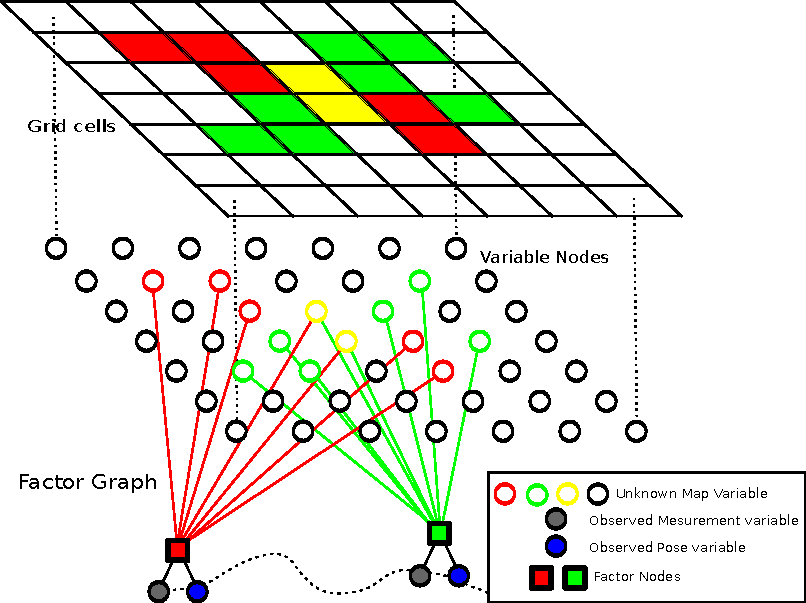
\includegraphics[trim=0in 0in 0in 0in, width=0.8\textwidth]{figures/factorgraph/factorgraph3.pdf}
\end{frame}

\begin{frame}
  \frametitle{Occupancy Grid to factor graph}
  \begin{itemize}
      \item $V$ = Map cells are variable nodes
      \item $F$ = Laser measurements are factor nodes
      \item E = $\{(i, f) : i \in V, f \in F, \text{laser $f$ passes through cell $i$}\}$
  \end{itemize}
  Posterior over the map can be factorized into forward sensor models
  \begin{align}
    P(\map) &= \frac{1}{Z}\prod_{f \in F} P_f(\map_f)
  \end{align}
\end{frame}

\begin{frame}
  \frametitle{Metropolis Hastings (Merali2013icra)}
  \begin{align}
    a = \frac{P(\map')Q(\map^r| \map')}
    {P(\map^r)Q(\map'| \map^r)}
  \end{align}
  \begin{align}
    Q(\map'| \map^r) = \begin{cases}
      \frac{1}{N} & \text{if $\|\map' - \map^r\|_1 = 1$}\\
                0 & \text{ otherwise}
    \end{cases}
    \label{eq:transitionprob}
  \end{align}
\end{frame}

\begin{comment}
\begin{frame}
  \frametitle{Metropolis Hatings}
  \begin{algorithm}
    \KwData{
      Factor Graph $G = (V, F, E)$\;
  %Label set $\{\Sx\}_{i \in V}$\;
  %Step size $\alpha > 0$\;
      Maximum number of iterations $N$\;
    }
    \KwResult{$\map^r$}
    Initialize the map $\map^0$ randomly.\;
    $r = 0$\;
    \While {$r < N$} {
      Randomly choose a cell $i : i \in V$\;
      Flip its state $x'_i = \neg x^r_i$ in $\map^r$ to get $\map'$\;
      Compute acceptance probability $a$ by \eqref{eq:acceptanceprob}\;
      Sample random number $q : 0 \le q \le 1$\;
      \If {$a \ge 1$ or $a \ge q$} {
        Accept proposed point, $\map^{r + 1} = \map'$\;
      } \Else {
        Reject proposed point, $\map^{r + 1} = \map^r$\;
      }
      $r \leftarrow r + 1$\;
    }
    \caption{Metropolis Hastings}
    \label{alg:metropolis}
  \end{algorithm}
\end{frame}
\end{comment}

\newcommand{\bpmsg}[4]{\mu^{#4}_{#1\rightarrow#2}(#3)}
\begin{frame}
  \frametitle{Sum product belief propagation}
  \begin{align}
    \bpmsg{f}{i}{l_i}{r+1} &= \sum_{\map_f \in \Omega_f: x_i = l_i}P_f(\map_f)\prod_{j \in n(f) \setminus i}\bpmsg{j}{f}{x_j}{r}
    \label{eq:factor2node}
    \\
    \bpmsg{i}{f}{l_i}{r+1} &= \prod_{h \in n(i) \setminus f}\bpmsg{h}{i}{l_i}{r}
    \label{eq:node2factor}
  \end{align}
\end{frame}

\newcommand{\msg}[3]{\mu_{#1#2}(#3)}
\newcommand{\assign}{\leftarrow}
\newcommand{\Sx}{L_i}
\begin{frame}
  \frametitle{Subgradient dual decomposition}
  \begin{algorithm}[H]
    \DontPrintSemicolon
    %\KwData{\;
    %  Factor Graph $G = (V, F, E)$\;
  %L%abel set $\{\Sx\}_{i \in V}$\;
    %  Step size $\alpha > 0$\;
    %  Maximum number of iterations $N$\;
    %}
    %\KwResult{Labels $\{x^f_i\}_{(i, f) \in E} $,
    %Messages $\{\msg{i}{f}{x_i}\}$}

    $\msg{i}{f}{x_i} \assign 0 \hfill \forall (i, f) \in E, x_i \in \Sx$\;
    $r \assign 1$\;
    \While{$r < N$} {
    %\tcp{For disagreeing factors}
      \For {$f \in F$} {% : \exists i, i' \in n(f) : x_i^f \ne x_{i'}^f$} {
        $\map^f \assign \argmin\limits_{\map^f} \left( \theta_f(\map^f) + \sum\limits_{i \in n(f)}\msg{i}{f}{x^f_i} \right)$\;
      %$\map^f \assign \argmax\limits_{\map^f} P_f(\map^f)
      %\prod\limits_{i \in n(f)}\exp\left(-\msg{i}{f}{x^f_i} \right)$\;
      }
      \tcp{For disagreeing nodes}
      \For {$i \in V : \exists f, f' \in n(i) : x_i^{f'} \ne x_i^f$} {
        \For{$f \in n(i)$}{
          $\msg{i}{f}{x^f_i} \assign \msg{i}{f}{x^f_i} + \frac{\alpha}{r}$\;
        }
      }
      $r \leftarrow r + 1$\;
    }
    %\caption{Subgradient Dual Decomposition}
    %\label{alg:dualdecomposition}
  \end{algorithm}
\end{frame}
% \begin{frame}
%   \frametitle{Notation}
%   \begin{itemize}
%       \item $\kappa_t = \kappa(z_t, x_t)$ = $[\kappa^i_t]_{i=1}^{n}$ \\
%         = List of $n$ cells that laser goes through for $t^{th}$ observation when travels for $z_t$ units.
%   \end{itemize}
%   \begin{figure}
%     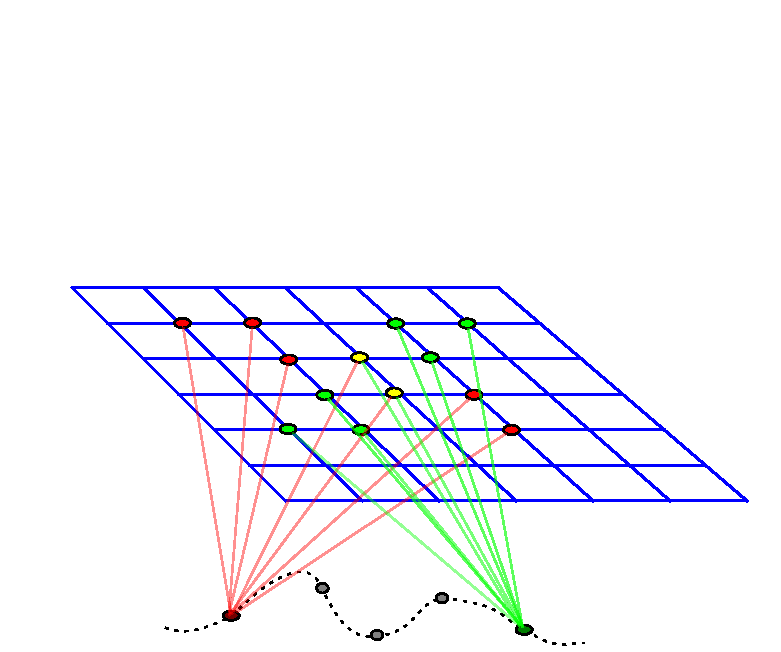
\includegraphics[trim=0in 0in 0in 2in, width=0.7\textwidth]{figures/factorgraph/fg3.pdf}
%   \end{figure}
% \end{frame}

\newcommand{\actz}{\bar{z}_f(\map_f, g_f)}
\begin{frame}
  \frametitle{Forward Sensor models}
  \begin{itemize}
      \item Gaussian sensor model
        \begin{align}
          p(z_f|\map_f, g_f) &=
          \frac{1}{\sqrt{2\pi}\sigma}\exp\left(-\frac{(\actz - z_f)^2}{2\sigma^2}\right)
          \label{eq:gaussiansensormodel}
        \end{align}
      \item Piecewise sensor model
        \begin{align}
          p(z_f|\map_f, g_f) &= \frac{1}{Z}\begin{cases}
                           1 & \text{ if } \map_f = [0, 0 \dots 0,
1]^\top\\
                  \exp(-900) & \text{ if } \map_f = [0, 0 \dots 0,
0]^\top\\
                 \exp(-1000) & \text{ otherwise}
        \end{cases}
        \label{eq:piecewiseconstant}
      \end{align}
  \end{itemize}
\end{frame}

\begin{frame}
  \frametitle{Higher order factors taken exponential time}
  \begin{itemize}
    \item Belief propagation
      \begin{align}
        \bpmsg{f}{i}{l_i}{r+1} &= \sum_{\map_f \in \Omega_f: x_i = l_i}P_f(\map_f)\prod_{j \in n(f) \setminus i}\bpmsg{j}{f}{x_j}{r}
      \end{align}
    \item Dual decomposition
      \begin{align}
        \map^f &= \argmin\limits_{\map^f} \theta_f(\map^f)
        +\sum\limits_{i \in n(f)}\msg{i}{f}{x^f_i}
      \end{align}
  \end{itemize}
\end{frame}

\begin{frame}
  \frametitle{Sensor models as Pattern based factors}
  \begin{align}
    P'_f(\map_f) = \begin{cases}
      \psi_{m} & \text{ if $\map_f \sim \vect{R}_m$} \,\,\, \forall 1 \le m \le M\\
    \psi_{\text{min}} & \text{ otherwise}
    \end{cases}
    \label{eq:patternfunction}
  \end{align}
  where $\vect{R}_m$ is of the form  $[r^m_1, r^m_2, *, r^m_3, *, *, *, r^m_4 \dots *]$. Let us call the fixed nodes (without star) be $n^m_0(f)$.
\end{frame}
\begin{frame}
  \frametitle{Efficient belief propagation}
  Instead of 
  \begin{align}
    \bpmsg{f}{i}{l_i}{r+1} &= \sum_{\map_f \in \Omega_f: x_i = l_i}P_f(\map_f)\prod_{j \in n(f) \setminus i}\bpmsg{j}{f}{x_j}{r}
  \end{align}
  We do:
  \begin{multline}
    p(\vect{x_f} \sim \vect{R}_m|x_i = l_i) \\
    = \begin{cases}
      0 & \text{if $i \in n^m_0(f)$ and $l_i \ne r^m_i$}\\
  \prod\limits_{j \in n^m_0(f) \setminus i}\bpmsg{j}{f}{r^m_j}{r} & \text{otherwise}
    \end{cases}
  \end{multline}
  \begin{multline}
    \bpmsg{f}{i}{l_i}{r+1} = \sum_{m \le M} \psi_m p(\vect{x_f} \sim \vect{R}_m|x_i = l_i)
    + \psi_{\text{min}} p_{\text{otherwise}}
    \label{eq:efficientbp}
  \end{multline}
  where $p_{\text{otherwise}} = 1 - \sum_{m \le M}p(\vect{x_f} \sim \vect{R}_m|x_i = l_i)$.
\end{frame}

\begin{frame}
  \frametitle{Efficient Dual decomposition}
  \begin{itemize}
      \item Find minimum of each pattern by taking the minimum message 
      \item Finding minimum of otherwise case, there are two cases
        \begin{itemize}
          \item If the otherwise can be enumerated efficienty, find the minimum over all enumerations
          \item Otherwise assume that the fixed patterns covered by the enumerated patterns are sparse. Find n-best maximas (or minimas) till the assignment do not coincides with enumerated patterns.
        \end{itemize}
      \item Find minimum among all the patterns
  \end{itemize}
\end{frame}

\begin{frame}
  
\includegraphics[width=0.16\textwidth]{../Data/cave_player/gt-final.png}%
  
\includegraphics[width=0.16\textwidth]{../Data/cave_player/TwoAssumptionAlgo.png}%
  
\includegraphics[width=0.16\textwidth]{../Data/cave_player/SICKSlowMetropolis.png}%
  
\includegraphics[width=0.16\textwidth]{../Data/cave_player/SICKDDMCMC.png}%
  
\includegraphics[width=0.16\textwidth]{../Data/cave_player/run_belief_propagation.png}%
  
\includegraphics[width=0.16\textwidth]{../Data/cave_player/dualdecomposition.png}\\
  
\includegraphics[width=0.16\textwidth]{../Data/hospital_player/gt-final.png}%
  
\includegraphics[width=0.16\textwidth]{../Data/hospital_player/TwoAssumptionAlgo.png}%
  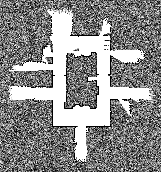
\includegraphics[width=0.16\textwidth]{../Data/hospital_player/SICKSlowMetropolis.png}%
  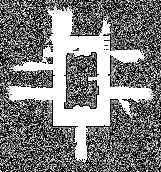
\includegraphics[width=0.16\textwidth]{../Data/hospital_player/SICKDDMCMC.png}%
  
\includegraphics[width=0.16\textwidth]{../Data/hospital_player/run_belief_propagation.png}%
  
\includegraphics[width=0.16\textwidth]{../Data/hospital_player/dualdecomposition.png}\\
  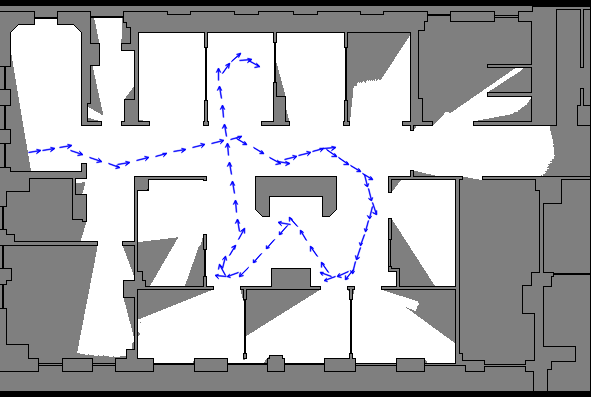
\includegraphics[width=0.16\textwidth]{../Data/hospital_section_player/trajectory-gt.png}%
  
\includegraphics[width=0.16\textwidth, trim=0 0 0 3px, clip]{../Data/hospital_section_player/TwoAssumptionAlgo.png}%
  
\includegraphics[width=0.16\textwidth, trim=0 0 0 3px, clip]{../Data/hospital_section_player/SICKSlowMetropolis.png}%
  
\includegraphics[width=0.16\textwidth, trim=0 0 0 3px, clip]{../Data/hospital_section_player/SICKDDMCMC.png}%
  
\includegraphics[width=0.16\textwidth, trim=0 0 0 3px, clip]{../Data/hospital_section_player/run_belief_propagation.png}%
  
\includegraphics[width=0.16\textwidth, trim=0 0 0 3px, clip]{../Data/hospital_section_player/dualdecomposition.png}\\
  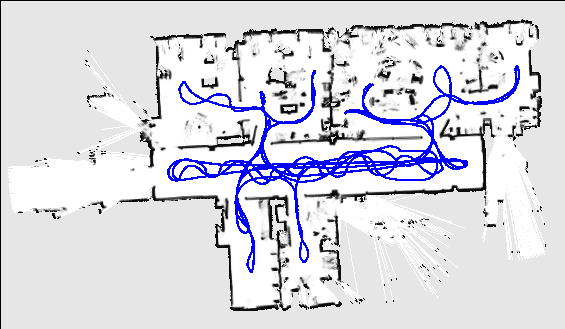
\includegraphics[height=0.16\textwidth, angle=90]{../Data/albertb.sm/path.png}%
  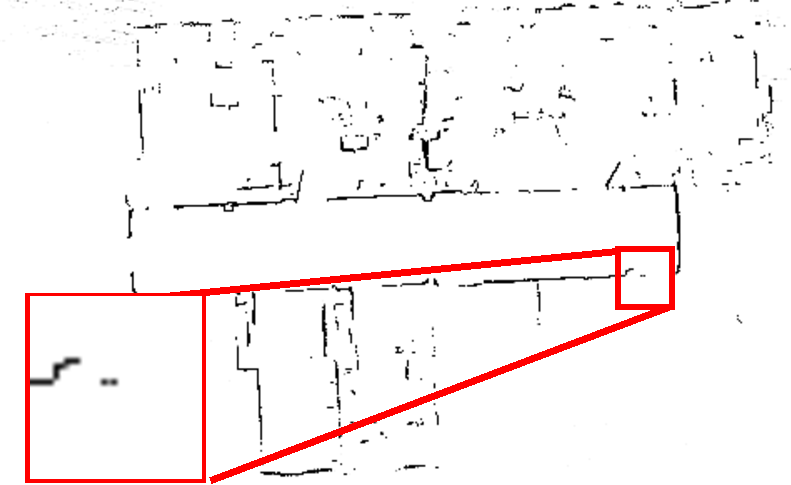
\includegraphics[height=0.16\textwidth, angle=90]{figures/zoomAndShow/zoomAndShowTwoAssumptionAlg.pdf}%
  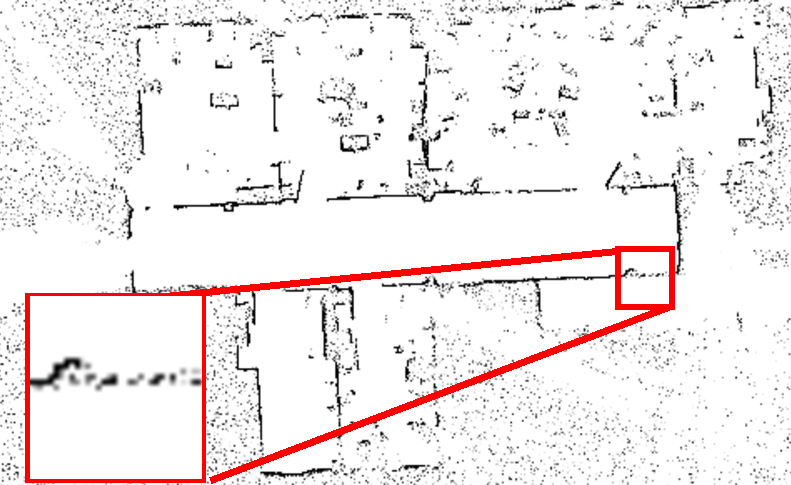
\includegraphics[height=0.16\textwidth, angle=90]{figures/zoomAndShow/zoomAndShowSICKDDMCMC.pdf}%
  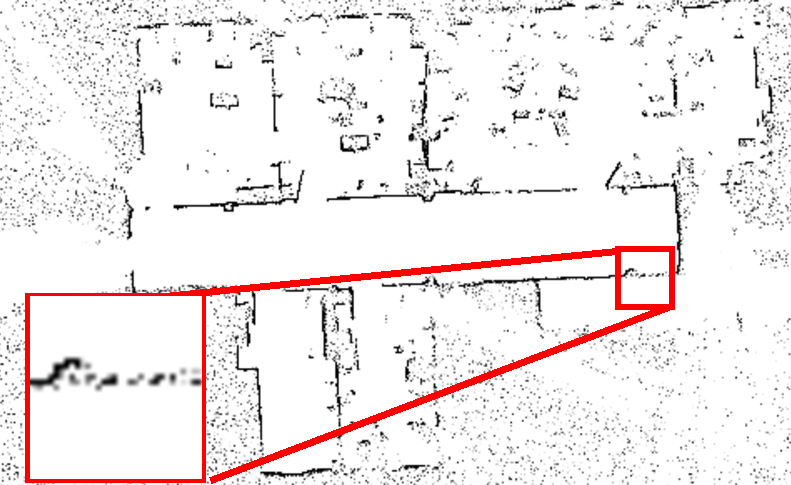
\includegraphics[height=0.16\textwidth, angle=90]{figures/zoomAndShow/zoomAndShowSICKDDMCMC.pdf}%
  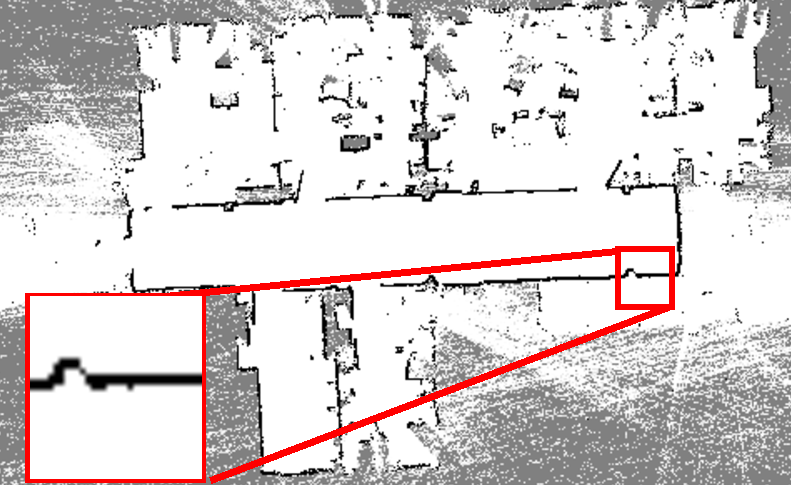
\includegraphics[height=0.16\textwidth, angle=90]{figures/zoomAndShow/zoomAndShowBP.pdf}%
  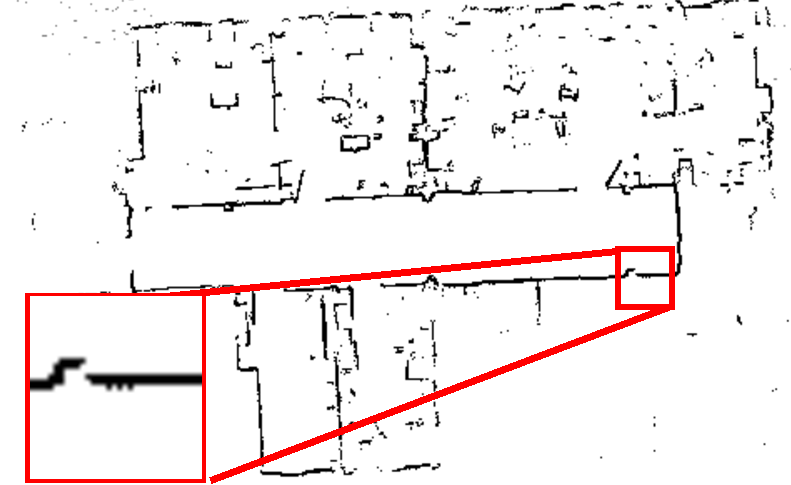
\includegraphics[height=0.16\textwidth, angle=90]{figures/zoomAndShow/zoomAndShowDD.pdf}%
\end{frame}

\begin{frame}
  \frametitle{Convergence of different algorithms}
\providecommand{\mysubfloatwidth}{0.50\textwidth}
%\begin{figure}
%  \subfloat[Convergence on cave dataset]{%
%    \label{subfig:convCave}%
  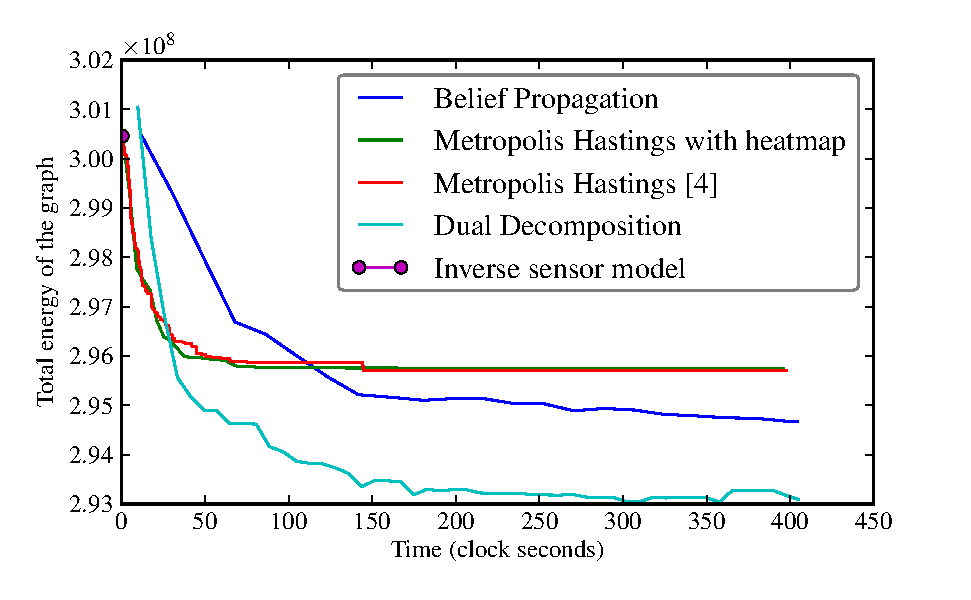
\includegraphics[width=\mysubfloatwidth]{../Data/cave_player/plot-time-energy.pdf}%
%}%
%  \subfloat[Convergence on hospital section dataset]{%
%    \label{subfig:convHospitalSection}%
  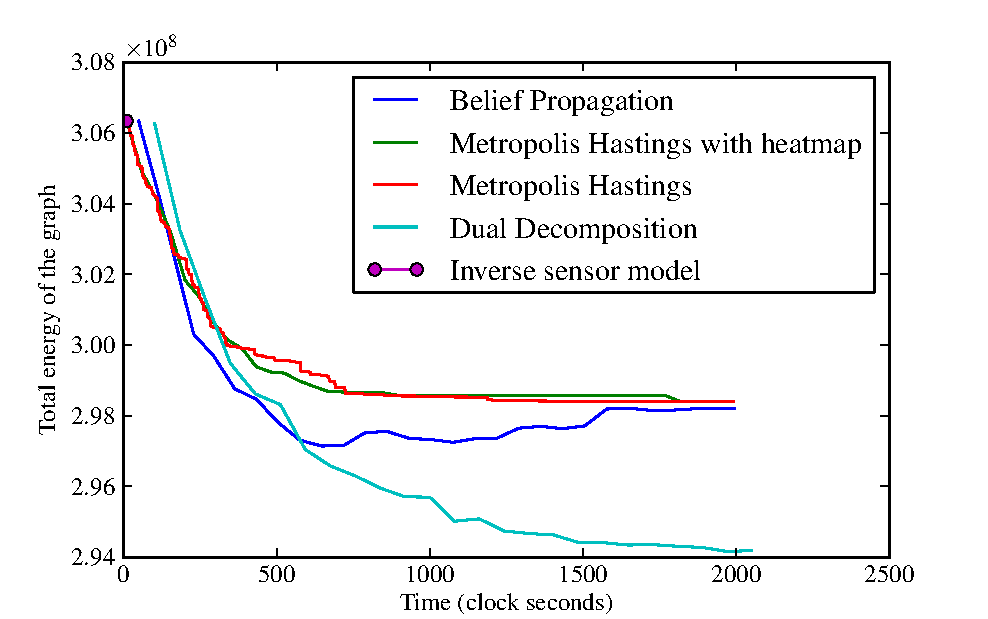
\includegraphics[width=\mysubfloatwidth]{../Data/hospital_section_player/plot-time-energy.pdf}\\
  %
%}%
  %\subfloat[Convergence on :TODO: dataset]{%
  %  \label{subfig:convTODO}%
  \includegraphics[width=\mysubfloatwidth]{../Data/hospital_player/plot-time-energy.pdf}%
%  \subfloat[Convergence on hospital dataset]{%
%    \label{subfig:convHospital}%
  %\includegraphics[width=\mysubfloatwidth]{../../Data/hospital_player/plot-time-energy.pdf}%
%}%
%  \subfloat[Convergence on albert-b dataset]{%
%    \label{subfig:convAlbert-b}%
  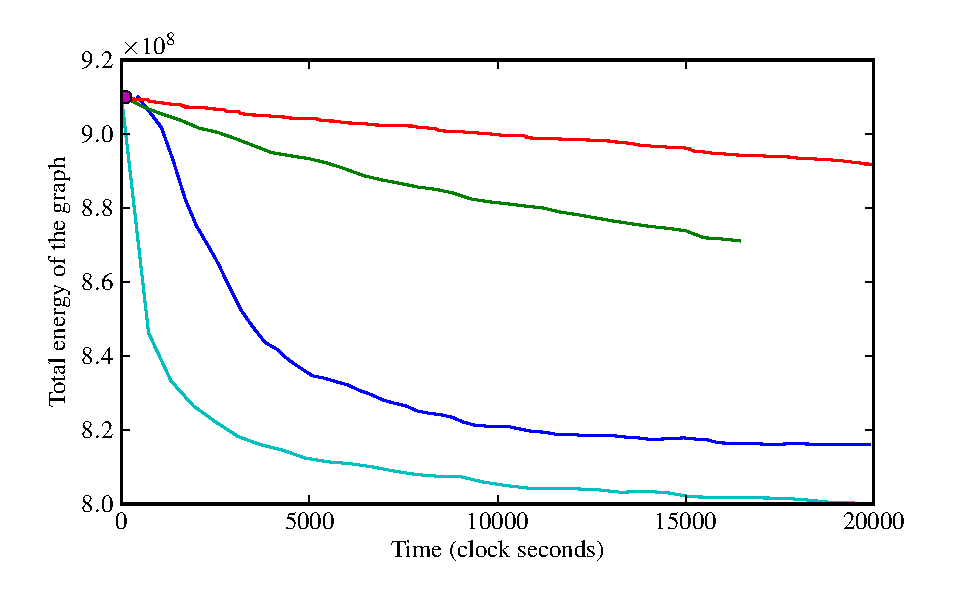
\includegraphics[width=\mysubfloatwidth]{../Data/albertb.sm/plot-time-energy.pdf}%
%}%
  %{Comparison of convergence rate of different algorithms on occupancy
  %  grid mapping. The left graph shows the convergence on simulated dataset
  %  \emph{cave}, while the right shows for \emph{albert-b}
  %  \cite{howard2003radish} dataset.  While sampling methods like Metropolis
  %  hastings converge quickly they stay far from optimum energy.  On the other
  %  hand modern inference algorithms like belief propagation and dual
  %  decomposition reach closer to an optimum value. The legends are listed
  %  only once for clarity.
    % While
    % \subref{subfig:convCave}-\subref{subfig:convAlbert-b} show convergence on different
    % datasets, \subref{fig:dualdecomposition-stepsize} shows the effect of step size on
    % convergence of dual decomposition algorithm.
  %}
  %\label{fig:convergence-comparison}
%\end{figure}
\end{frame}

\begin{comment}
\begin{frame}
  \frametitle{Factorization (Brian's technique)}
  \begin{align}
    p(m_k|z, x, m_{neg k}) &= \frac{1}{Z} p(m_k|m_{\neg k}) \prod_t p(z_t|m, x_t)\\
                           &= \frac{1}{Z} p(m_k|m_{\neg k}) \prod_t p(z_t|m_{\kappa_t}, x_t)\\
  p(z_t|m_{\kappa_t}, x_t) &= \frac{1}{Z'}exp(-E(m_{\kappa_t}, z_t, x_t))\\
  E(m_{\kappa_t}, z_t, x_t) &= \begin{cases}
              0 & \text{if $m_{k} = 0 \forall k \in \{\kappa^i_t\}_{i=1}^{n-1} \land m_{\kappa_t^n} = 1$}\\
            900 & \text{if $m_{k} = 0 \forall k \in \{\kappa^i_t\}_{i=1}^{n-1} \land m_{\kappa_t^n} = 0$}\\
           1000 & \text{ otherwise}
    \end{cases}
  \end{align}

\end{frame}
\begin{frame}
  \begin{figure}
    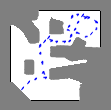
\includegraphics[width=0.3\textwidth]{figures/cave_gt.png}
    
\includegraphics[width=0.3\textwidth]{figures/mcmc_100x100.png}
    
\includegraphics[width=0.3\textwidth]{figures/two-assumption_100x100.png}
    \caption{From left to right: 1) Observed ground truth (resolution: 500x500) 2) Gibbs sampling merali2013icra $20 \times 10^4$ samples(resolution:100x100) 3) Two-assumption method (resolution:500x500) }
    \label{fig:results}
  \end{figure}
\end{frame}

\begin{frame}
  With occupancy prior 0.5
  \begin{figure}
    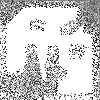
\includegraphics[width=0.3\textwidth]{figures/Metropolis_Marginals_20k_iter.png}
    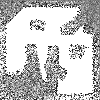
\includegraphics[width=0.3\textwidth]{figures/Metropolis_Marginals_40k_iter.png}
    
\includegraphics[width=0.3\textwidth]{figures/metropolis_100x100.png}
    \caption{From left to right: Marginals computed by metropolis hastings algorithm with 1) $2 \times 10^4$ samples (resolution:100x100) 2) with $4 \times 10^4$ samples and 3) with $10 \times 10^4$ samples }
    \label{fig:metropolis-results}
  \end{figure}
\end{frame}

\begin{frame}
  With occupancy prior 0.3
  \begin{figure}
    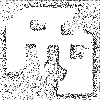
\includegraphics[width=0.3\textwidth]{figures/occgridvis200.png}
    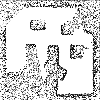
\includegraphics[width=0.3\textwidth]{figures/occgridvis400.png}
    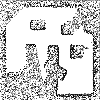
\includegraphics[width=0.3\textwidth]{figures/occgridvis600.png}
    \caption{From left to right: Marginals computed by metropolis hastings algorithm with 1) $2 \times 10^4$ samples (resolution:100x100) 2) with $4 \times 10^4$ samples and 3) with $6 \times 10^4$ samples }
    \label{fig:metropolis-results}
  \end{figure}
\end{frame}

\begin{frame}
  With occupancy prior 0.3 and resolution 200x200.
  \begin{figure}
    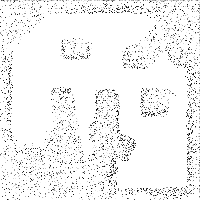
\includegraphics[width=0.3\textwidth]{figures/occgridvis200_200x200.png}
    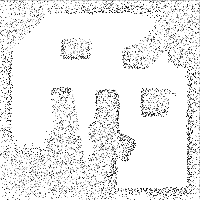
\includegraphics[width=0.3\textwidth]{figures/occgridvis400_200x200.png}
    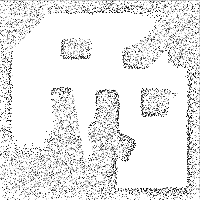
\includegraphics[width=0.3\textwidth]{figures/occgridvis600_200x200.png}
    \caption{From left to right: Marginals computed by metropolis hastings algorithm with 1) $2 \times 10^4$ samples (resolution:100x100) 2) with $4 \times 10^4$ samples and 3) with $6 \times 10^4$ samples }
    \label{fig:metropolis-results}
  \end{figure}
\end{frame}
    
\end{comment}

\end{document}
